\documentclass[../lecture-notes.tex]{subfiles}

\begin{document}

\subsection{Commitments}

\begin{definition}
    A cryptographic commitment scheme allows one party to commit to a chosen statement (such as a value, vector, or polynomial) without revealing the statement itself. The commitment can be revealed in full or in part at a later time, ensuring the integrity and secrecy of the original statement until the moment of disclosure.
\end{definition}

Imagine putting a letter into a box and locking it with your key. 
You then give that box to your friend, who cannot open it without the key.
In this scenario, you have made a commitment to the letter inside the box. 
You cannot change the content of the letter, as it is in your friend's possession. 
At the same time, your friend cannot access the letter since they do not have the key to unlock the box.

% \begin{center}
%     \centering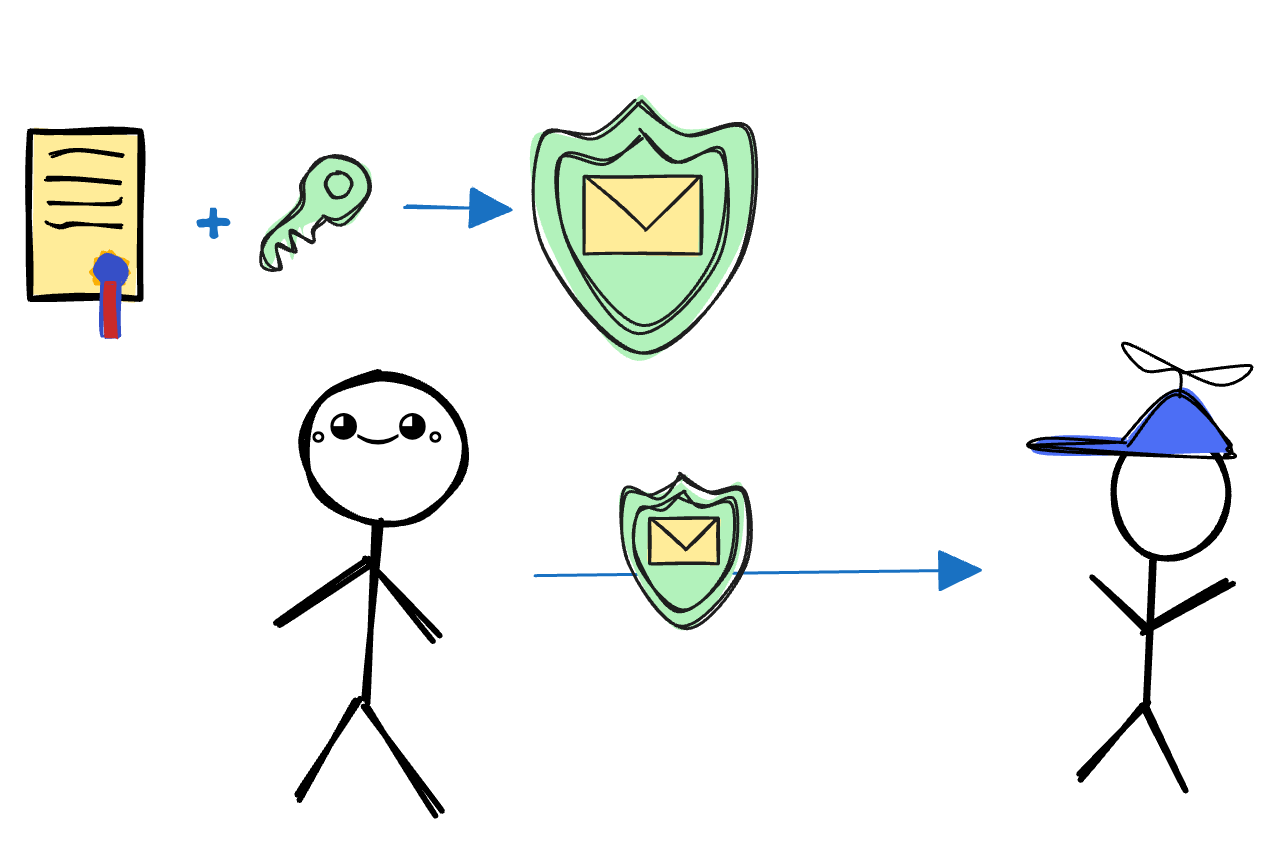
\includegraphics[width=0.5\linewidth, clip]{images/lecture_5/CommitmentExample.png}

%     \scriptsize{\textbf{Illustration:} Commitment scheme}
% \end{center}

Commitment scheme has 3 stages:
\begin{enumerate}
    \item \textit{Setup:}  prover and verifier agree on common parameters before the commitment process begins;

    \item \textit{Commit:} prover selects a value and generates a commitment to this value. This commitment is then sent to the verifier;

    \item  \textit{Verify:} prover reveals the committed value and any necessary information to the verifier. 
\end{enumerate}

Properties of commitments scheme:
\begin{enumerate}
    \item \textit{Hiding: } verifier should not learn any information about the message given only the commitment c;
    \item \textit{Binding: } prover could not find another message $m_1$ and open the commitment $c$ without revealing the commited message $m$.
\end{enumerate}

\subsubsection{Hash-based commitments}

As the name implies, we are using a cryptographic hash function \(H\) in such scheme.

\begin{enumerate}
    \item Prover selects a message $m$ which he wants to commit:
        $m \leftarrow \mathbb{Z}$

    \item Prover samples random value $r$ (usually called blinding factor) from $\mathbb{Z}$:
        $r \xleftarrow{R} \mathbb{Z}$
    
    \item Both values will be concatenated and hashed with the hash function $H$ to produce the commitment:
        $c = H(m || r)$

\end{enumerate}

Commitment should be shared with a verifier. During the verification stage, prover reveals $(m, r)$ to the verifier. 
To check the commitment, verifier computes: $c_1 = H(m || r)$.

If $c_1 = c$, prover has revealed the correct pair $(m, r)$.

\subsubsection{Pedersen commitments}

Pedersen commitments allow us to represent arbitrarily large vectors with a single elliptic curve point, while optionally hiding any information about the vector. Pedersen commitment uses a public group $\mathbb{G}$ of order $q$ and two random public generators $G$ and $U$: $U = uG$. Secret parameter $u$ should be hidden, otherwise the $\textit{Binding}$ property of the commitment scheme will be violated.
EC point $U$ is chosen randomly using "Nothing-up-my-sleeve" to assure no one knows the discrete logorithm of a selected point.
Pedersen commitment scheme algorithm:
\begin{enumerate}
    \item 
\end{enumerate}


\subsubsection{Vector commitments}

Vector commitments




\end{document}